\subsection{自我介绍}

\begin{frame}{自我介绍}
    \begin{columns}
        % col 1
        \column{0.3\textwidth}

        \center \large{赵华男}

        \begin{figure}
            \centering
            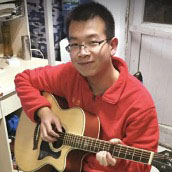
\includegraphics[width=3cm]{Images/自我介绍1.jpg}
        \end{figure}

        \begin{block}{\tiny{研究方向}}
            \small{生物信息学 | 基因编辑}
        \end{block}
        \bigskip
        \bigskip
        \bigskip
        \bigskip
        \bigskip
        \bigskip
        \bigskip
        \bigskip
        \bigskip
        \bigskip
        \bigskip
        \bigskip
        % col 2
        \column{0.7\textwidth}

        \begin{block}{\tiny{学习经历}}
            \begin{itemize}
                % \tiny
                \item {2014 $ \sim $ 2019 \quad 西北农林科技大学(学士)}
                \item {2016 $ \sim $ 2018 \quad 中国农业大学 (交换生)}
                \item {2019 $ \sim $ 至今 \quad 清华大学 博士研究生(PTN项目)}
                \item {2020 $ \sim $ 至今 \quad 北京大学 (联合培养)}
            \end{itemize}
        \end{block}
        \begin{columns}
            \column{0.4\textwidth}
            \begin{figure}
                \centering
                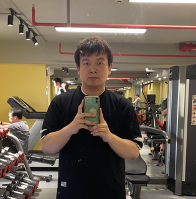
\includegraphics[width=3cm]{Images/自我介绍2.png}
            \end{figure}
            \column{0.4\textwidth}
            \begin{figure}
                \centering
                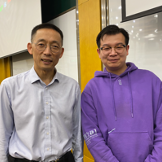
\includegraphics[width=3cm]{Images/自我介绍3.png}
            \end{figure}
        \end{columns}


        \bigskip
        \bigskip
        \bigskip
        \bigskip
        \bigskip
        \bigskip
        \bigskip
        \bigskip
        \bigskip
        \bigskip
    \end{columns}
\end{frame}
% 大家好!
% 今天是 2022-09-11 日
% 非常高兴能够作为主讲人给大家讲授这门
% 利用 Python 进行生信分析 的课程

% 在开始课程介绍之前,
% 首先请允许我做一个简短的自我介绍,也方便大家认识我
% 我叫赵华男
% 我在 2014 年参加高考,考入西北农林科技大学
% 在 2019 年,我从西北农林科技大学毕业,拿到了我的学士学位
% 期间我作为交换生在中国农业大学学习并顺利结业
% 在 2019 年,我通过北京大学,清华大学和北京生命科学研究所的联合招生项目
% 也就是 PTN 项目, 来到清华大学生命科学学院攻读博士学位
% 一年之后,也就是 2020, 我最终定导在北京大学我导师的实验室
% 我的研究方向呢,是生物信息学与基因编辑
% 好, 闲话少聊,我们开始这门课程的第一节,课程介绍
\subsection{课程介绍}
\begin{frame}[standout] 第一节 \quad 课程介绍 \end{frame}



\begin{frame}{这门课的开设目的}
    教大家使用 Python 写程序
    \begin{figure}
        \centering
        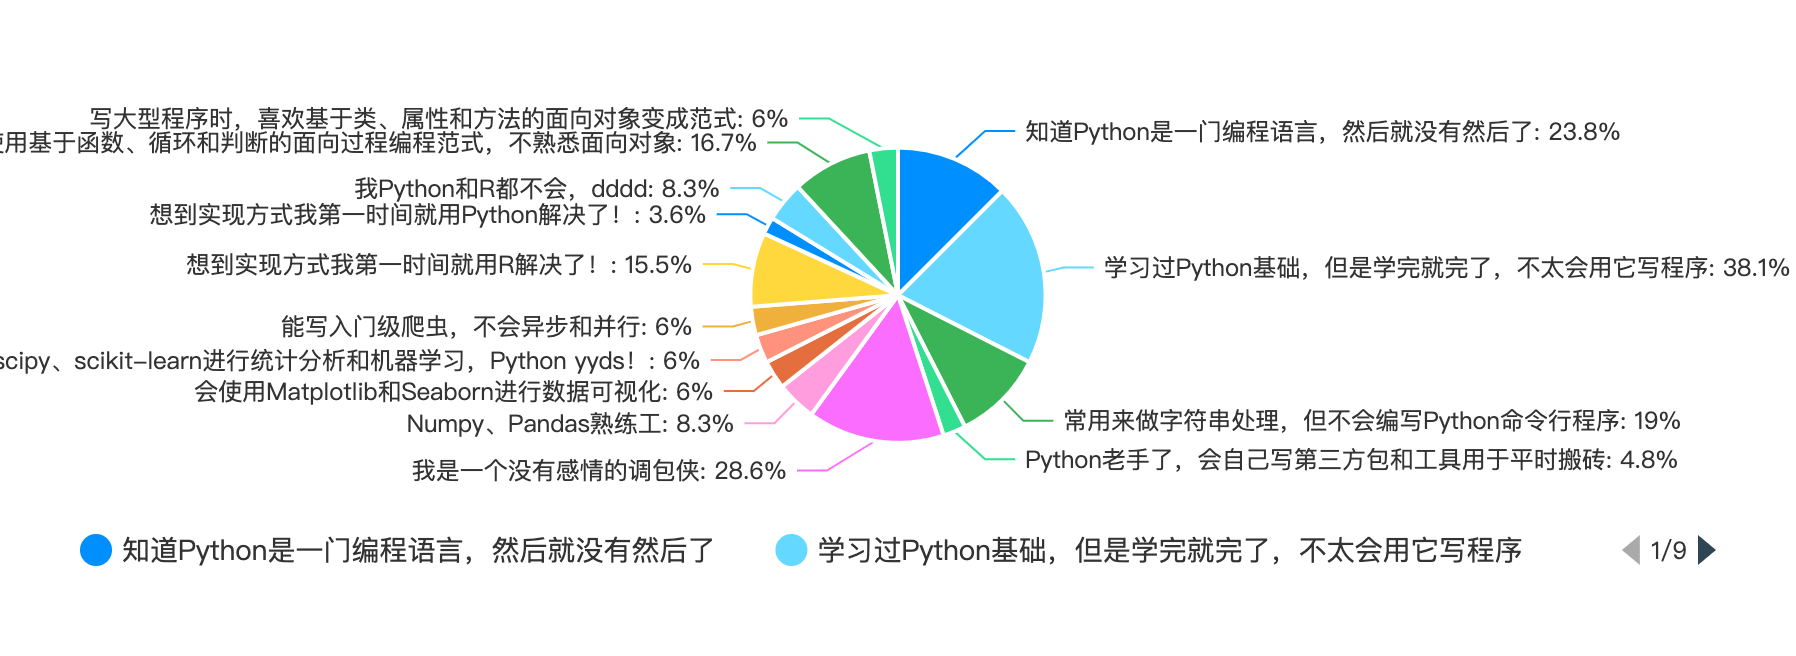
\includegraphics[width=15cm]{Images/level.png}
    \end{figure}
\end{frame}

% 正如课程介绍页面所述,这门课程的核心目的是教大家用 Python 写程序


\begin{frame}{这门课的开设目的}
    教大家使用 Python 写程序
    \begin{figure}
        \centering
        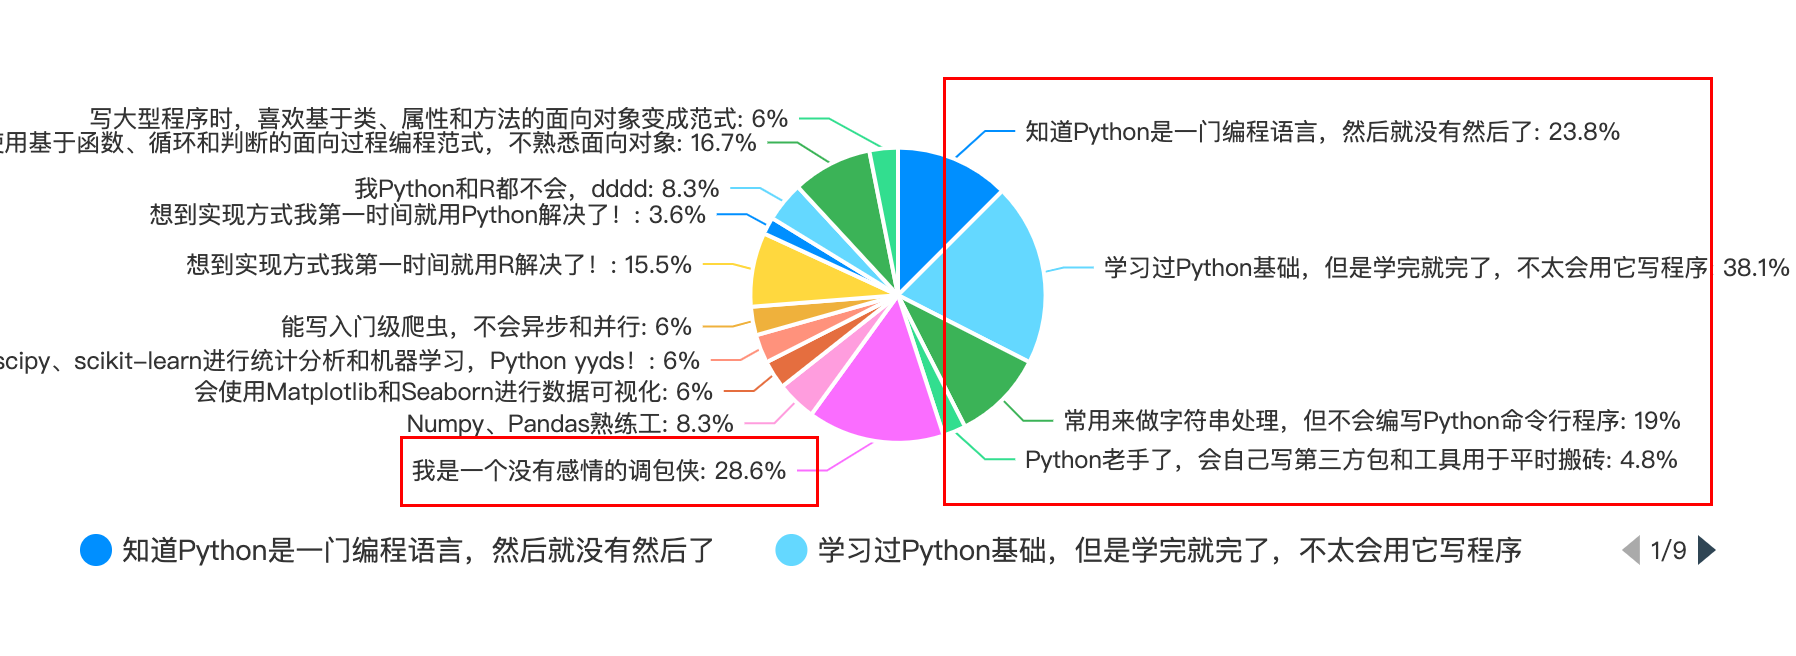
\includegraphics[width=15cm]{Images/level2.png}
    \end{figure}
\end{frame}
% 这张饼图是我做的一个问卷调查表,大家可以看到,
% 23.8%的同学没有学习过 Python
% 但是接近 40%的同学学习过 Python,但是并不会用它写程序
% 这门课程的目的,是为了解决大家关于 Python 学了不会用的痛点
% 或着是大家会用一些第三方包,但是 Python 使用和理解不够深入的问题


\begin{frame}{这门课的开设目的}
    教大家使用 Python 写程序 → 基础 + 有难度的几个实战项目
    \begin{figure}
        \centering
        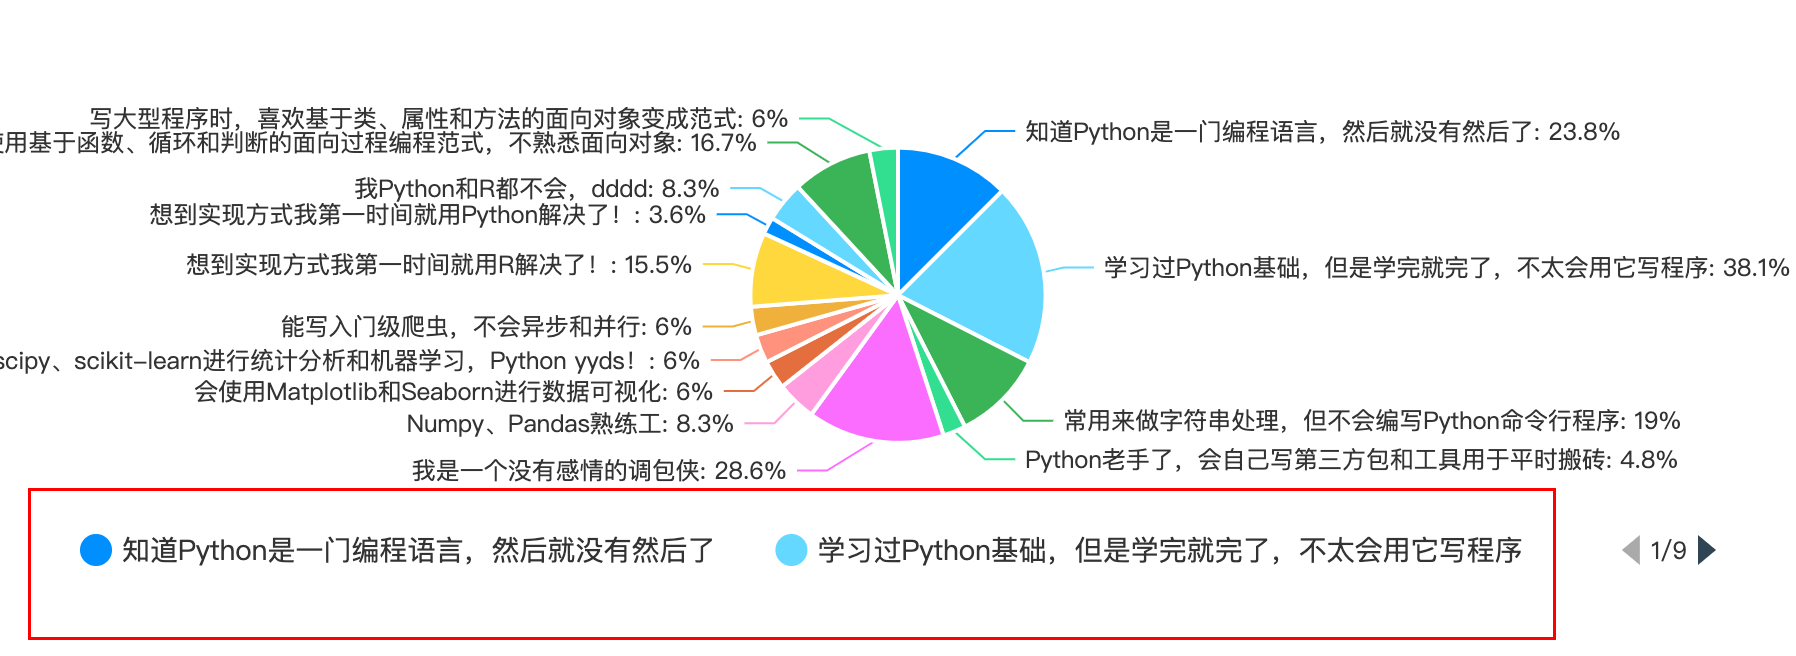
\includegraphics[width=15cm]{Images/level3.png}
    \end{figure}
\end{frame}

% 那这门课程, 我将会带着大家,用大量的时间,
% 使用 Python 完成几个比较有难度的生物信息学编程开发项目,
% 当然, 为了照顾一些零基础的同学,我们也将在课程一开始,
% 介绍操作系统的基本概念和 Python 的基础知识

% 我们先来看一下这门课程的设计思路

\begin{frame}{课程设计}
    \begin{itemize}
        \item 操作系统和编程语言 (Shell, PATH)
        \item Python 基础知识 + Python 进阶知识
        \item 编程实战(核心)
        \begin{itemize}
            \item 序列文件的处理(FASTA, FASTQ)
            \item BED 文件的操作与处理(BED)
            \item 基因注释文件处理(GFF, GTF)
            \item BAM 文件的解析与操作(SAM, BAM)
            \item 支持多核计算程序的编写
            \item 复杂命令行工具的编写与搭建
        \end{itemize}
    \end{itemize}
\end{frame}

% 首先,这是一门编程课,我们避免不了的要接触Linux 和命令行,
% 所以我们会简略地介绍一下操作系统和环境配置,和几个简单的 SHELL 命令,以及环境变量
% 接下来,我们将从 Python 的基础知识讲起, 过渡到Python进阶知识,也就是面向对象的一些概念
% 然后进入本课程的核心部分,编程实战,
% 在这个部分,我们针对生物信息学中常见的文件和分析需求,设计了六大实战模块
% 认真跟下来这几个项目,我相信大家
% 不但能获得项目开发能力的提高
% 还可以树立生物信息学分析的信心,针对常见分析需求,能够做到自信自己能搞定,成竹在胸

\begin{frame}[standout] Thank you! \end{frame}
% 好的,我们的第一节 课程介绍,就已经讲完了, 非常欢迎大家和我一起学习接下来的内容


